% Created 2020-07-22 mié 10:40
% Intended LaTeX compiler: pdflatex
\documentclass[presentation,aspectratio=169]{beamer}
\usepackage[utf8]{inputenc}
\usepackage[T1]{fontenc}
\usepackage{graphicx}
\usepackage{grffile}
\usepackage{longtable}
\usepackage{wrapfig}
\usepackage{rotating}
\usepackage[normalem]{ulem}
\usepackage{amsmath}
\usepackage{textcomp}
\usepackage{amssymb}
\usepackage{capt-of}
\usepackage{hyperref}
\usepackage{khpreamble}
\usepackage{amssymb}
\usepackage{pgfplotstable}
\DeclareMathOperator{\shift}{q}
\DeclareMathOperator{\diff}{p}
\usetheme{default}
\author{Kjartan Halvorsen}
\date{\today}
\title{Control computarizado - Identificación de sistemas}
\hypersetup{
 pdfauthor={Kjartan Halvorsen},
 pdftitle={Control computarizado - Identificación de sistemas},
 pdfkeywords={},
 pdfsubject={},
 pdfcreator={Emacs 26.3 (Org mode 9.3.6)}, 
 pdflang={English}}
\begin{document}

\maketitle

\section{Retroalimentacion Examen parcial 2}
\label{sec:org77514cb}

\begin{frame}[label={sec:org3ee4b09}]{Retroalimentación Examen parcial 2}
\begin{itemize}
\item La mayoridad dominan bien un gran parte de la materia
\item Dos cosas a enforzar
\begin{enumerate}
\item Interpretación de funciones de transferencia (diagrama de Bode)
\item Transformar especifiaciones en el tiempo a ubicación de los polos
\end{enumerate}
\end{itemize}
\end{frame}

\begin{frame}[label={sec:orgbd3c51f}]{Retroalimentación Examen parcial 2 - funciones de transferencia}
\begin{center}
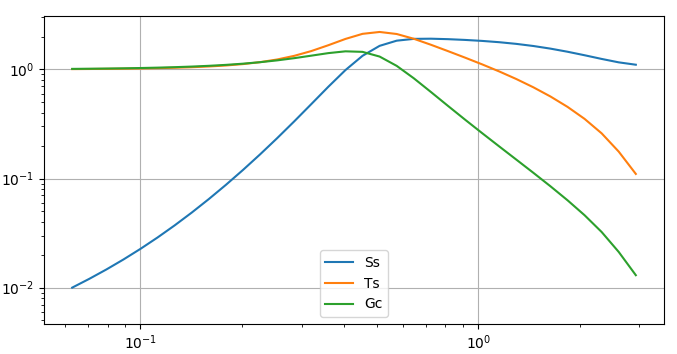
\includegraphics[width=0.7\linewidth]{../../figures/sensitivity-fcn-bode-example.png}
\end{center}
\end{frame}

\begin{frame}[label={sec:org389d856}]{Retroalimentación Examen parcial 2 - Ubicación de polos}
Dado \(h=0.01\), y usando \(t_s \approx \frac{4}{\zeta\omega_n} < 0.01\)
\[z = \mathrm{e}^{sh} = \mathrm{e}^{\text{Re}(s)h} \mathrm{e}^{i\text{Im}(s)h}\]
\[|z| = |\mathrm{e}^{sh}| = |\mathrm{e}^{\text{Re}(s)h}| < \mathrm{e}^{-\zeta\omega_n h} = \mathrm{e}^{-40\cdot 0.01} = 0.67\]   
\begin{center}
\alert{plano s} \hspace*{0.4\linewidth} \alert{plano z}\\
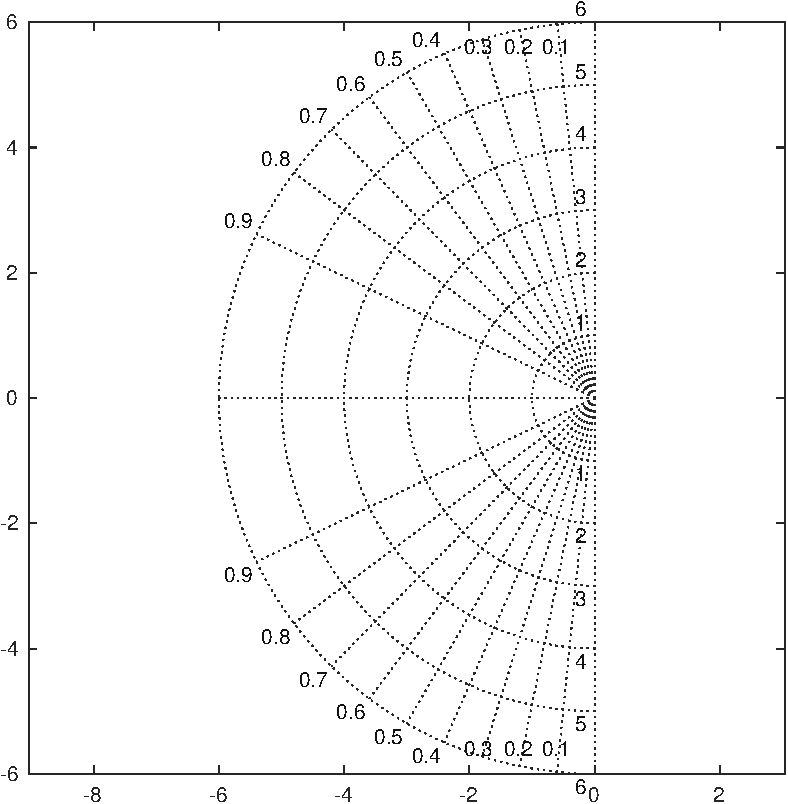
\includegraphics[height=0.61\textheight]{../../figures/sgrid-crop} \hspace*{3mm}
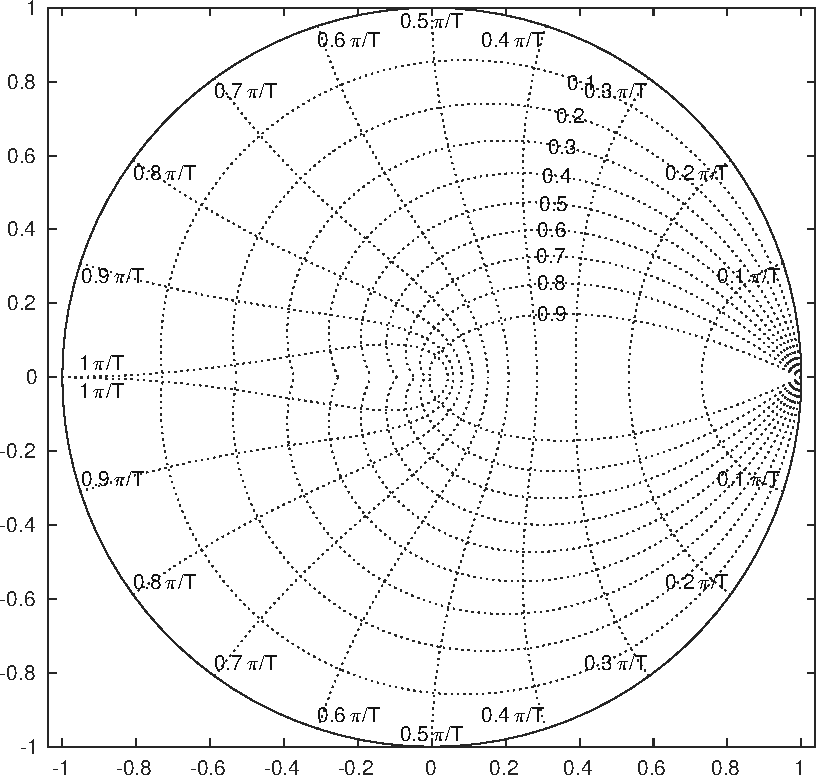
\includegraphics[height=0.6\textheight]{../../figures/zgrid-crop}\\
\end{center}
\end{frame}


\section{Intro}
\label{sec:org6e42a51}
\begin{frame}[label={sec:orgace4d88}]{Identificación de sistemas}
\end{frame}
\begin{frame}[label={sec:org56108b1}]{Identificación de sistemas}
\def\uampl{0.5}
\def\ttdelay{0.3}
\def\TTcnst{1.6}
\def\ggain{3}
\def\tdelay{1.125} % Resulting from method
\def\Tcnst{2.625} % Resulting from method

\pgfmathsetmacro{\yfinal}{\uampl*\ggain}
\pgfmathsetmacro{\yone}{0.283*\yfinal}
\pgfmathsetmacro{\ytwo}{0.632*\yfinal}
\pgfmathsetmacro{\tone}{2}
\pgfmathsetmacro{\two}{3.75}


\begin{center}
  \begin{tikzpicture}
    \begin{axis}[
    width=12cm,
    height=5.5cm,
    %grid = both,
    minor y tick num=9,
    minor x tick num=9,
    every major grid/.style={red, opacity=0.5},
    xlabel = {$t$},
    xmin = -1,
    clip=false,
    ]
      \addplot [thick, green!50!black, no marks, domain=0:10, smooth, samples=16] {\uampl*\ggain*(x>\ttdelay)*(1 - (1+(x-\ttdelay)/\TTcnst)*exp(-(x-\ttdelay)/\TTcnst))} node [coordinate, pos=0.9, pin=-90:{$y(t)$}] {};
      \addplot [const plot, thick, blue!80!black, no marks, domain=-1:10, samples=100] coordinates {(-1,0) (0,0) (0,\uampl) (10,\uampl)} node [coordinate, pos=0.9, pin=-90:{$u(t)$}] {};
      \addplot [thick, olive!80!black, smooth, no marks, domain=0:10, samples=100] {\uampl*\ggain*(x>\tdelay)*(1 - exp(-(x-\tdelay)/\Tcnst)} node [coordinate, pos=0.6, pin=-90:{$G=\ggain\frac{\mathrm{e}^{-\tdelay s}}{s\Tcnst + 1}$}] {};
      \draw[thick, red, dashed] (axis cs: \tone, \yone) -- (axis cs: \tone, -0.45) node[below] {$t_1 = \tone = \tau + \frac{T}{3}$}; 
      \draw[thick, red, dashed] (axis cs: \tone, \yone) -- (axis cs: -2,\yone) node[left, anchor=east] {$0.283y_f = \yone$}; 
      \draw[thick, orange, dashed] (axis cs: \two, \ytwo) -- (axis cs: \two, -0.9) node[below] {$t_2 = \two = \tau + T$}; 
      \draw[thick, orange, dashed] (axis cs: \two, \ytwo) -- (axis cs: -2, \ytwo, -0.9) node[left, anchor=east] {$0.632y_f = \ytwo$}; 
      \draw[thick, green!60!black, dashed] (axis cs: 10, \yfinal) -- (axis cs: -2, \yfinal) node[left, anchor=east] {$y_f = \yfinal$}; 
      \draw[blue!70!black, dashed] (axis cs: 10, \uampl) -- (axis cs: 10.2, \uampl, -0.9) node[above] {$u_f = \uampl$}; 

    \end{axis}
  \end{tikzpicture}
\end{center}
\end{frame}


\begin{frame}[label={sec:orge542e13}]{Identificación de sistemas}
\begin{center}
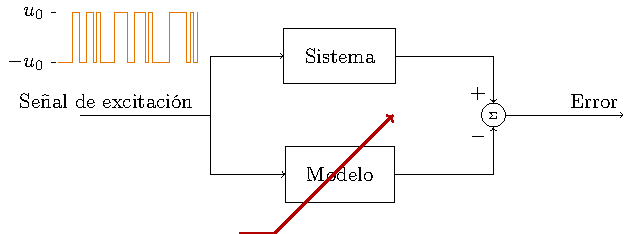
\includegraphics[]{sysid-graphic} 
\end{center}
\end{frame}

\section{AR-model}
\label{sec:org6a036c8}

\begin{frame}[label={sec:org6a7e686}]{Ejemplo - Modelo autoregresivo (AR)}
\end{frame}
\begin{frame}[label={sec:org3e73b75}]{Modelo autoregresivo (AR)}
Dado una secuencia discreta observada \(y(k), \; k=1,2,\ldots,N\), y el modelo autoregresivo
\[ y(k+1) = -ay(k) + e(k+1),\]
dónde \(e(k)\) es una sequencia discreta de ruido blanco.

\alert{Objetivo} Estimar el parametro \(a\).

\begin{enumerate}
\item Forma el predictor de un paso adelante \[\hat{y}_{k+1} = -ay_k=-y_ka = \varphi_{k+1} \theta,\] y el error de predicción \[\epsilon_k = y_k - \hat{y}_k = y_k - \varphi_k \theta\]
\end{enumerate}
\end{frame}


\begin{frame}[label={sec:org831e949}]{Modelo autoregresivo (AR)}
Dado una secuencia discreta observada \(y(k), \; k=1,2,\ldots,N\), y el modelo autoregresivo
\(y(k+1) = -ay(k) + e(k+1),\)
dónde \(e(k)\) es una sequencia discreta de ruido blanco.

\alert{Objetivo} Estimar el parametro \(a\).

\begin{enumerate}
\setcounter{enumi}{1}
\item Reune todas las observaciónes \(y_k\) y predicciones \(\hat{y}_k\) en forma vectoral
\begin{align*}
\epsilon &= \begin{bmatrix} \epsilon_2\\\epsilon_2\\\vdots\\\epsilon_N\end{bmatrix} =  \begin{bmatrix} y_2\\ y_3\\\vdots\\y_N \end{bmatrix} - \begin{bmatrix} \hat{y}_2\\ \hat{y}_3\\\vdots\\\hat{y}_N \end{bmatrix}
 =  \begin{bmatrix} y_2\\ y_3\\\vdots\\y_N \end{bmatrix} - \begin{bmatrix} -y_1 a\\ -y_2 a\\\vdots\\-y_{N-1}^T\theta \end{bmatrix} =  \begin{bmatrix} y_2\\ y_3\\\vdots\\y_N \end{bmatrix} - \begin{bmatrix} \varphi_2^T\theta\\ \varphi_3^T\theta\\\vdots\\\varphi_N^T\theta \end{bmatrix}\\
&= y - \underbrace{\begin{bmatrix}\varphi_1^T\\\varphi_2^T\\\vdots\\\varphi_N^T\end{bmatrix}}_{\Phi}\theta = y - \Phi\theta 
\end{align*}
\end{enumerate}
\end{frame}



\begin{frame}[label={sec:org6451f54}]{Modelo autoregresivo (AR)}
Dado una secuencia discreta observada \(y(k), \; k=1,2,\ldots,N\), y el modelo autoregresivo
\(y(k+1) = -ay(k) + e(k+1),\)
dónde \(e(k)\) es una sequencia discreta de ruido blanco.

\alert{Objetivo} Estimar el parametro \(a\).

\begin{enumerate}
\setcounter{enumi}{2}
\item Obtiene el estimado de mínimos cuadrados 
\begin{align*}
 \theta_{LS} &= (\Phi^T\Phi)^{-1}\Phi^T y\\ &= \left(\begin{bmatrix} -y_1 & -y_2 & \cdots & -y_{N-1}\end{bmatrix}\begin{bmatrix}-y_1\\-y_2\\\vdots\\-y_{N-1}\end{bmatrix}\right)^{-1}\begin{bmatrix} -y_1 & -y_2 & \cdots & -y_{N-1}\end{bmatrix}\begin{bmatrix}y_2\\y_3\\\vdots\\y_N\end{bmatrix}\\
 &= -\frac{\sum_{k=1}^{N-1} y_ky_{k+1}}{\sum_{k=1}^{N-1}y_k^2}
 \end{align*}
\end{enumerate}
\end{frame}


\begin{frame}[label={sec:org04aa7cb},fragile]{Computación de la solución de mínimos cuadrados}
 Dado error de predicción en forma vectoral para sistema de orden \(n\)
\(\epsilon = y - \Phi\theta\). Forma el sistema de ecuaciones
\begin{align*}
\Phi \theta &= y\\
\begin{bmatrix}\varphi_{n+1}^T\\\varphi_{n+2}^T\\\varphi_{n+3}^T\\\varphi_{n+4}^T\\\vdots\\\varphi_{N}^T\end{bmatrix} \begin{bmatrix}\theta_1\\\theta_2\\\vdots\\\theta_m\end{bmatrix} &= \begin{bmatrix}y_{n+1}\\y_{n+2}\\y{n+3}\\y_{n+4}\\\vdots\\ y_{N}\end{bmatrix}
\end{align*}
Resuelva las ecuaciones usando métodos numericamente robustos de algebra lineal, por ejemplo   factorización L-U. En matlab se escribe
\begin{verbatim}
theta_LS = Phi \ y
\end{verbatim}
\end{frame}

\begin{frame}[label={sec:orgd135160}]{Ejemplo numerico}
\href{https://mybinder.org/v2/gh/kjartan-at-tec/mr2007-computerized-control/master?filepath=.\%2Fsystem-identification\%2Fnotebooks\%2FAR-example.ipynb}{Mybinder}
\end{frame}



\begin{frame}[label={sec:orgd1882dd}]{Model AR de orden \(n\)}
Dado una secuencia discreta observada \(y(k), \; k=1,2,\ldots,N\), y el modelo autoregresivo
\begin{align*} 
A(z)Y(z) = z^nE(z) \quad \Leftrightarrow \quad A(\shift)y(k) &= \shift^{n-1} e(k)\\
(\shift^n + a_1\shift^{n-1} + a_2\shift^{n-2} + \cdots + a_n)y(k) &= \shift^n e(k)\\
(\shift + a_1 + a_2\shift{-1} + \cdots + a_n\shift^{-n+1})y(k) &= \shift e(k)\\
y(k+1) + a_1y(k)  + a_2y(k-1) + \cdots + a_ny(k-n+1) &= e(k+1)\\
y(k+1) = -a_1y(k)  - a_2y(k-1) - \cdots - a_ny(k-n+1) &+ e(k+1)
\end{align*}
dónde \(e(k)\) es una sequencia discreta de ruido blanco.

\alert{Objetivo} Estimar los parametro \(a_1, a_2, \ldots, \a_n\).
\end{frame}


\begin{frame}[label={sec:org68a1fb7}]{Model AR de orden \(n\)}
Dado una secuencia discreta observada \(y(k), \; k=1,2,\ldots,N\), y el modelo autoregresivo
\(y(k+1) = -a_1y(k)  - a_2y(k-1) - \cdots - a_ny(k-n+1) + e(k+1)\).

\begin{enumerate}
\item Forma el predictor de un paso adelante 
\[\hat{y}_{k+1} = -a_1y_k-a_2y_{k-1} - \ldots - a_n y_{k-n+1}a = \underbrace{\begin{bmatrix} -y_{k} & -y_{k-1} & \cdots & -y_{k-n+1}\end{bmatrix}}_{\varphi_{k+1}^T}\underbrace{\begin{bmatrix}a_1\\a_2\\\vdots\\a_n\end{bmatrix}}_{\theta}\]
y el error de predicción \[\epsilon_k = y_k - \hat{y}_k = y_k - \varphi_k^T \theta\]
\end{enumerate}
\end{frame}

\begin{frame}[label={sec:orgc1b932b}]{Model AR de orden \(n\)}
Dado una secuencia discreta observada \(y(k), \; k=1,2,\ldots,N\), y el modelo autoregresivo
\(y(k+1) = -a_1y(k)  - a_2y(k-1) - \cdots - a_ny(k-n+1) + e(k+1)\).

\begin{enumerate}
\setcounter{enumi}{1}
\item Reune todas las observaciónes \(y_k\) y predicciones \(\hat{y}_k\) en forma vectoral
\begin{align*}
\epsilon &= \begin{bmatrix} \epsilon_{n+1}\\\epsilon_{n+2}\\\vdots\\\epsilon_N\end{bmatrix} =  \begin{bmatrix} y_{n+1}\\ y_{n+2}\\\vdots\\y_N \end{bmatrix} - \begin{bmatrix} \hat{y}_{n+1}\\ \hat{y}_{n+2}\\\vdots\\\hat{y}_N \end{bmatrix}
 =  \begin{bmatrix} y_{n+1}\\ y_{n+2}\\\vdots\\y_N \end{bmatrix} - \begin{bmatrix} \varphi_{n+1}^T\theta\\ \varphi_{n+2}^T\theta\\\vdots\\\varphi_N^T\theta \end{bmatrix}\\
&= y - \underbrace{\begin{bmatrix}\varphi_{n+1}^T\\\varphi_{n+2}^T\\\vdots\\\varphi_N^T\end{bmatrix}}_{\Phi}\theta = y - \Phi\theta 
\end{align*}
\end{enumerate}
\end{frame}

\begin{frame}[label={sec:org85dbae9}]{Model AR de orden \(n\)}
Dado una secuencia discreta observada \(y(k), \; k=1,2,\ldots,N\), y el modelo autoregresivo
\(y(k+1) = -a_1y(k)  - a_2y(k-1) - \cdots - a_ny(k-n+1) + e(k+1)\).
\begin{enumerate}
\setcounter{enumi}{2}
\item Obtiene el estimado de mínimos cuadrados, que es
\begin{align*}
 \theta_{LS} &= (\Phi^T\Phi)^{-1}\Phi^T y
 \end{align*}
formando y resolviendo el sistema de ecuaciones
\begin{align*}
\Phi \theta &= y\\
\begin{bmatrix}\varphi_{n+1}^T\\\varphi_{n+2}^T\\\varphi_{n+3}^T\\\varphi_{n+4}^T\\\vdots\\\varphi_{N}^T\end{bmatrix} \begin{bmatrix}a_1\\a_2\\\vdots\\a_n\end{bmatrix} &= \begin{bmatrix}y_{n+1}\\y_{n+2}\\y_{n+3}\\y_{n+4}\\\vdots\\ y_{N}\end{bmatrix}
\end{align*}
\end{enumerate}
\end{frame}


\begin{frame}[label={sec:org8b127ba}]{Modelo autoregresivo (AR) - Ejercicio}
Dado una secuencia discreta observada \(y(k), \; k=1,2,\ldots,N\), y el modelo autoregresivo de segunda orden
\[ y(k+2) + a_1y(k+1) + a_2y(k) = e(k+2),\]
dónde \(e(k)\) es una sequencia discreta de ruido blanco.

\alert{Actividad} Forma las ecuaciones \[ \Phi \theta = y\]
\end{frame}


\section{ARX-model}
\label{sec:orgd32a1f9}

\begin{frame}[label={sec:org0f113e6}]{Model AutoRegresivo con variables eXógenas (ARX)}
Dado señal discreta de entrada de un sistema \(u(k), \; k=1,2,\ldots, N\) y observaciones de la respuesta \(y(k), \; k=1,2,\ldots,N\), y el modelo ARX
\[ A(\shift) y(k) = B(\shift)u(k) + e(k+n),\]
dónde \(e(k)\) es una sequencia discreta de ruido blanco.

\alert{Actividad} Llena los bloques

\begin{center}
  \begin{tikzpicture}[node distance=22mm, block/.style={rectangle, draw, minimum width=15mm, minimum height=12mm}, sumnode/.style={circle, draw, inner sep=2pt}]
    
    \node[coordinate] (input) {};
    \node[block, right of=input, node distance=20mm] (plant)  {};
    \node[sumnode, right of=plant, node distance=24mm] (sum) {\tiny $\Sigma$};
    \node[block, above of=sum, node distance=20mm] (dist)  {};

    \node[coordinate, above of=dist, node distance=12mm] (disturbance) {};
    \node[coordinate, right of=sum, node distance=20mm] (output) {};

    \draw[->] (input) -- node[above, pos=0.3] {$u(k)$} (plant);
    \draw[->] (plant) -- node[above] {} (sum);
    \draw[->] (sum) -- node[above, near end] {$y(k)$} (output);
    \draw[->] (disturbance) -- node[right, pos=0.2] {$e(k)$} (dist);
    \draw[->] (dist) -- node[above] {} (sum);

  \end{tikzpicture}
\end{center}
\end{frame}


\begin{frame}[label={sec:orgac6cf2d}]{Model AutoRegresivo con variables eXógenas (ARX) - solución}
\end{frame}
\begin{frame}[label={sec:org57dc41c}]{Model AutoRegresivo con variables eXógenas (ARX) - solución}
Dado señal discreta de entrada de un sistema \(u(k), \; k=1,2,\ldots, N\) y observaciones de la respuesta \(y(k), \; k=1,2,\ldots,N\), y el modelo ARX
\[ A(\shift) y(k) = B(\shift)u(k) + e(k+n),\]
dónde \(e(k)\) es una sequencia discreta de ruido blanco.
\begin{center}
  \begin{tikzpicture}[node distance=22mm, block/.style={rectangle, draw, minimum width=15mm, minimum height=12mm}, sumnode/.style={circle, draw, inner sep=2pt}]
    
    \node[coordinate] (input) {};
    \node[block, right of=input, node distance=20mm] (plant)  {$\frac{B(z)}{A(z)}$};
    \node[sumnode, right of=plant, node distance=24mm] (sum) {\tiny $\Sigma$};
    \node[block, above of=sum, node distance=20mm] (dist)  {$\frac{z^n}{A(z)}$};

    \node[coordinate, above of=dist, node distance=12mm] (disturbance) {};
    \node[coordinate, right of=sum, node distance=20mm] (output) {};

    \draw[->] (input) -- node[above, pos=0.3] {$u(k)$} (plant);
    \draw[->] (plant) -- node[above] {} (sum);
    \draw[->] (sum) -- node[above, near end] {$y(k)$} (output);
    \draw[->] (disturbance) -- node[right, pos=0.2] {$e(k)$} (dist);
    \draw[->] (dist) -- node[above] {} (sum);

  \end{tikzpicture}
\end{center}
\end{frame}



\section{Esta parte el miercoles}
\label{sec:orgb8acce3}
\begin{frame}[label={sec:org4bcdcf6}]{Model ARX de orden \(n\)}
Dado señal discreta de entrada de un sistema \(u(k), \; k=1,2,\ldots, N\) y observaciones de la respuesta \(y(k), \; k=1,2,\ldots,N\), y el modelo ARX \(A(\shift)y(k) = B(\shift)u(k-d) + \shift^n e(k)\) con \(n\) polos, \(m\) ceros y retraso de \(d\) pasos
\[A(z)Y(z) = B(z)z^{-d}U(z) + z^nE(z) \quad \Leftrightarrow \quad A(\shift)y(k) = B(\shift)\shift^{-d}u(k) + \shift^{n} e(k)\]
\end{frame}

\begin{frame}[label={sec:org51226c5}]{Model ARX de orden \(n\)}
Dado señal discreta de entrada de un sistema \(u(k), \; k=1,2,\ldots, N\) y observaciones de la respuesta \(y(k), \; k=1,2,\ldots,N\), y el modelo ARX \(A(\shift)y(k) = B(\shift)u(k-d) + \shift^n e(k)\) con \(n\) polos, \(m\) ceros y retraso de \(d\) pasos
\[A(z)Y(z) = B(z)z^{-d}U(z) + z^nE(z) \quad \Leftrightarrow \quad A(\shift)y(k) = B(\shift)\shift^{-d}u(k) + \shift^{n} e(k)\]
\begin{multline*}
(\shift^n + a_1\shift^{n-1} + a_2\shift^{n-2} + \cdots + a_n)y(k) = (b_0\shift^{m-d} + b_1\shift^{m-d-1} + \cdots + b_m\shift^{-d})u(k)\\ +  \shift^n e(k)
\end{multline*}

\alert{Objetivo} Estimar los parametro \(a_1, a_2, \ldots, \a_n, b_0, b_1, \ldots, b_m\).
\end{frame}


\begin{frame}[label={sec:orgd4b900d}]{Model ARX de orden \(n\)}
\[A(z)Y(z) = B(z)z^{-d}U(z) + z^nE(z) \quad \Leftrightarrow \quad A(\shift)y(k) = B(\shift)\shift^{-d}u(k) + \shift^{n} e(k)\]
\begin{multline*}
(\shift^n + a_1\shift^{n-1} + a_2\shift^{n-2} + \cdots + a_n)y(k) = (b_0\shift^{m-d} + b_1\shift^{m-d-1} + \cdots + b_m\shift^{-d})u(k)\\ +  \shift^n e(k)
\end{multline*}
\begin{multline*}
(\shift + a_1 + a_2\shift^{-1} + \cdots + a_n\shift^{-n+1})y(k) = \\(b_0\shift^{m-n+1} + b_1\shift^{m-n} + \cdots + b_m\shift^{-n+1})\shift^{-d}u(k) +  \shift e(k)\\
\end{multline*}
\end{frame}

\begin{frame}[label={sec:org564c31d}]{Model ARX de orden \(n\)}
\[A(z)Y(z) = B(z)z^{-d}U(z) + z^nE(z) \quad \Leftrightarrow \quad A(\shift)y(k) = B(\shift)\shift^{-d}u(k) + \shift^{n} e(k)\]
\begin{multline*}
(\shift^n + a_1\shift^{n-1} + a_2\shift^{n-2} + \cdots + a_n)y(k) = (b_0\shift^{m-d} + b_1\shift^{m-d-1} + \cdots + b_m\shift^{-d})u(k)\\ +  \shift^n e(k)
\end{multline*}
\begin{multline*}
(\shift + a_1 + a_2\shift^{-1} + \cdots + a_n\shift^{-n+1})y(k) = \\(b_0\shift^{m-n+1} + b_1\shift^{m-n} + \cdots + b_m\shift^{-n+1})\shift^{-d}u(k) +  \shift e(k)\\
\end{multline*}
\begin{multline*}
y(k+1) = -a_1y(k) - \cdots - a_ny(k-n+1) \\+ b_0u(k+m-n-d+1) + \cdots + b_mu(k-n-d+1)  +   e(k+1)
\end{multline*}
\end{frame}

\begin{frame}[label={sec:org61f3817}]{Model ARX de orden \(n\)}
Dado señal discreta de entrada de un sistema \(u(k), \; k=1,2,\ldots, N\) y observaciones de la respuesta \(y(k), \; k=1,2,\ldots,N\), el modelo ARX \(A(\shift)y(k) = B(\shift)u(k-d) + \shift^n e(k)\) con \(n\) polos, \(m\) ceros y retraso de \(d\) pasos

\alert{Predictor}
\begin{multline*}
\hat{y}(k+1) = -a_1y(k) - \cdots - a_ny(k-n+1) \\+ b_0u(k+m-n-d+1) + \cdots + b_mu(k-n-d+1)  +   e(k+1)
\end{multline*}


\alert{Objetivo} Estimar los parametro \(a_1, a_2, \ldots, \a_n, b_0, b_1, \ldots, b_m\).
\end{frame}

\begin{frame}[label={sec:orgc8a22f0}]{Ejemplo y tarea}
\href{https://mybinder.org/v2/gh/kjartan-at-tec/mr2007-computerized-control/master?filepath=.system-identification\%2Fnotebooks\%2FParameter\%20estimation\%20with\%20least\%20squares\%20-\%20Homework.ipynb}{Mybinder}
\end{frame}
\end{document}